\documentclass{article}

% Language setting
\usepackage[brazil]{babel}

% Set page size and margins
\usepackage[a4paper,top=2cm,bottom=2cm,left=3cm,right=3cm,marginparwidth=1.75cm]{geometry}

% Useful packages
\usepackage{amsmath}
\usepackage{booktabs}
\usepackage{graphicx}
\usepackage{authblk}
\usepackage{minted}
\usepackage{svg}
\usepackage{blindtext}
\usepackage{titlesec}
\graphicspath{ {figures/} }
\usepackage{array}

\usepackage[colorlinks=true, allcolors=blue]{hyperref}

\title{ATIVIDADE PRÁTICA - ÁRVORE DE DECISÃO}
\author[1]{Jadson Goulart de Matos (21103270)}
\author[2]{Luan Daniel de Oliveira Melo (20102096)}
\affil[1]{DEC0014-06655 (20231) - Inteligência Artificial e Computacional, UFSC}

\begin{document}
\maketitle

\begin{abstract}
Uma árvore de decisão é um tipo de algoritmo de aprendizado de máquina supervisionado que pode lidar com variáveis numéricas e categóricas. Nesta atividade, a biblioteca scikit-learn foi utilizada para implementar a árvore de decisão em Python. O objetivo é prever se vai chover amanhã ou não, com base nessas variáveis.
\end{abstract}

\listoffigures
\listoftables
\newpage

\section{Introdução}
Nesta atividade prática, carregamos e limpamos os dados meteorológicos, codificamos variáveis categóricas, dividimos os dados em conjuntos de treinamento e teste, criamos e treinamos um modelo de árvore de decisão e avaliamos o desempenho do modelo.

Após o pré-processamento dos dados e a codificação das variáveis categóricas, preparamos a variável alvo codificando a coluna 'RainTomorrow'. Em seguida, procedeu-se ao treinamento do modelo de árvore de decisão usando os dados de treinamento.

Finalmente, avaliamos o desempenho do modelo calculando seu escore de precisão nos dados de treinamento. O modelo alcançou uma precisão de 81%.

Para desenvolver a solução de aprendizado de máquina baseada em Árvore de Decisão para classificar se vai chover amanhã ou não, com base em dados meteorológicos.

Árvore de decisão é um tipo de algoritmo de aprendizado de máquina supervisionado que pode lidar com variáveis numéricas e categóricas. Nessa atividade foi usado a biblioteca \cite{scikit-learn} scikit-learn para implementar da árvore de decisão em Python.

\section{Dados}
Os dados foram obtidos do Kaggle: \cite{Deekshitulu_2023}.

\begin{itemize}
  \item \textbf{Data}: A data da observação do tempo.
  \item \textbf{Localização}: O local onde os dados meteorológicos foram registrados.
  \item \textbf{MinTemp}: A temperatura mínima registrada nesse dia, que é de em graus Celsius.
  \item \textbf{MaxTemp}: A temperatura máxima registrada nesse dia, que é de em graus Celsius.
  \item \textbf{Precipitação}: A quantidade de chuva medida em milímetros, que é em mm.
  \item \textbf{Evaporação}: A quantidade de água evaporada do solo ou de outras superfícies durante o dia.
  \item \textbf{Sol}: O número de horas de sol registradas durante o dia.
  \item \textbf{WindGustDir}: A direção de onde se originou a rajada de vento mais forte, neste caso.
  \item \textbf{WindGustSpeed}: A velocidade da rajada de vento mais forte medida em quilômetros por hora, que é em km/h.
  \item \textbf{WindDir9am}: A direção do vento às 9h.
  \item \textbf{WindDir3pm}: A direção do vento às 3h.
  \item \textbf{WindSpeed9h}: A velocidade do vento às 9h, que é em km/h.
  \item \textbf{WindSpeed3h}: A velocidade do vento às 3h, que é em km/h.
  \item \textbf{Umidade9h}: A umidade relativa do ar às 9h, que é em \%.
  \item \textbf{Umidade3h}: A umidade relativa do ar às 3h, que é em \%.
  \item \textbf{Pressão9h}: A pressão atmosférica às 9h, que é em hPa.
  \item \textbf{Pressão3h}: A pressão atmosférica às 3h, que é em hPa.
  \item \textbf{Nuvens9h}: A fração de céu coberta por nuvens às 9h.
  \item \textbf{Nuvens3h}: A fração do céu coberta de nuvens às 3h.
  \item \textbf{Temp9am}: A temperatura às 9h, que é em graus Celsius.
  \item \textbf{Temp3pm}: A temperatura às 3h, que é em graus Celsius.
  \item \textbf{ChuvaHoje}: Indica se choveu naquele dia (Sim) ou não (Não).
  \item \textbf{RISK\_MM}: A quantidade de chuva registrada em milímetros para o dia seguinte. É uma medida do risco ou possibilidade de chuva.
  \item \textbf{RainTomorrow}: Indica se choveu no dia seguinte (Sim) ou não (Não).
\end{itemize}

Na primeira parte, é carregado os dados meteorológicos do arquivo CSV. Os dados contêm informações sobre a localização, data, temperatura, umidade, vento, chuva e outras variáveis meteorológicas de várias cidades da Austrália. O objetivo é prever se vai chover amanhã ou não, com base nessas variáveis. A coluna 'RainTomorrow' é a variável de destino.

\subsection{Visualização dos dados}
Antes de prosseguir para a criação e treinamento do modelo de árvore de decisão, é útil visualizar os dados para entender melhor as relações entre as variáveis.

\begin{table}[!ht]
  \resizebox{\columnwidth}{!}{%
  \begin{tabular}{lllllllllllllllllllllllll}
        & Date       & Location      & MinTemp & MaxTemp & Rainfall & Evaporation & Sunshine & WindGustDir & WindGustSpeed & WindDir9am & WindDir3pm & WindSpeed9am & WindSpeed3pm & Humidity9am & Humidity3pm & Pressure9am & Pressure3pm & Cloud9am & Cloud3pm & Temp9am & Temp3pm & RainToday & RISK\_MM & RainTomorrow \\
  0     & 2008-12-01 & Albury        & 13.4    & 22.9    & 0.6      &             &          & W           & 44.0          & W          & WNW        & 20.0         & 24.0         & 71.0        & 22.0        & 1007.7      & 1007.1      & 8.0      &          & 16.9    & 21.8    & No        & 0.0      & No           \\
  1     & 2008-12-02 & Albury        & 7.4     & 25.1    & 0.0      &             &          & WNW         & 44.0          & NNW        & WSW        & 4.0          & 22.0         & 44.0        & 25.0        & 1010.6      & 1007.8      &          &          & 17.2    & 24.3    & No        & 0.0      & No           \\
  2     & 2008-12-03 & Albury        & 12.9    & 25.7    & 0.0      &             &          & WSW         & 46.0          & W          & WSW        & 19.0         & 26.0         & 38.0        & 30.0        & 1007.6      & 1008.7      &          & 2.0      & 21.0    & 23.2    & No        & 0.0      & No           \\
  3     & 2008-12-04 & Albury        & 9.2     & 28.0    & 0.0      &             &          & NE          & 24.0          & SE         & E          & 11.0         & 9.0          & 45.0        & 16.0        & 1017.6      & 1012.8      &          &          & 18.1    & 26.5    & No        & 1.0      & No           \\
  4     & 2008-12-05 & Albury        & 17.5    & 32.3    & 1.0      &             &          & W           & 41.0          & ENE        & NW         & 7.0          & 20.0         & 82.0        & 33.0        & 1010.8      & 1006.0      & 7.0      & 8.0      & 17.8    & 29.7    & No        & 0.2      & No           \\
  5     & 2008-12-06 & Albury        & 14.6    & 29.7    & 0.2      &             &          & WNW         & 56.0          & W          & W          & 19.0         & 24.0         & 55.0        & 23.0        & 1009.2      & 1005.4      &          &          & 20.6    & 28.9    & No        & 0.0      & No           \\
  6     & 2008-12-07 & Albury        & 14.3    & 25.0    & 0.0      &             &          & W           & 50.0          & SW         & W          & 20.0         & 24.0         & 49.0        & 19.0        & 1009.6      & 1008.2      & 1.0      &          & 18.1    & 24.6    & No        & 0.0      & No           \\
  7     & 2008-12-08 & Albury        & 7.7     & 26.7    & 0.0      &             &          & W           & 35.0          & SSE        & W          & 6.0          & 17.0         & 48.0        & 19.0        & 1013.4      & 1010.1      &          &          & 16.3    & 25.5    & No        & 0.0      & No           \\
  5939  & 2009-01-01 & Cobar         & 17.9    & 35.2    & 0.0      & 12.0        & 12.3     & SSW         & 48.0          & ENE        & SW         & 6.0          & 20.0         & 20.0        & 13.0        & 1006.3      & 1004.4      & 2.0      & 5.0      & 26.6    & 33.4    & No        & 0.0      & No           \\
  23199 & 2016-04-26 & NorfolkIsland & 19.0    & 22.9    & 6.6      & 4.0         & 8.0      & SE          & 52.0          & ESE        & ESE        & 28.0         & 26.0         & 67.0        & 68.0        & 1021.0      & 1019.6      & 3.0      & 4.0      & 20.6    & 20.9    & Yes       & 0.0      & No           \\
  24999 & 2013-03-13 & Penrith       & 15.4    & 30.9    & 0.0      &             &          & NE          & 24.0          & NE         & NE         & 4.0          & 11.0         & 88.0        & 39.0        &             &             &          &          & 20.0    & 30.3    & No        & 0.0      & No          
  \end{tabular}%
  }
\caption{Amostra de todos os dados do CSV}
\end{table}

\begin{figure}
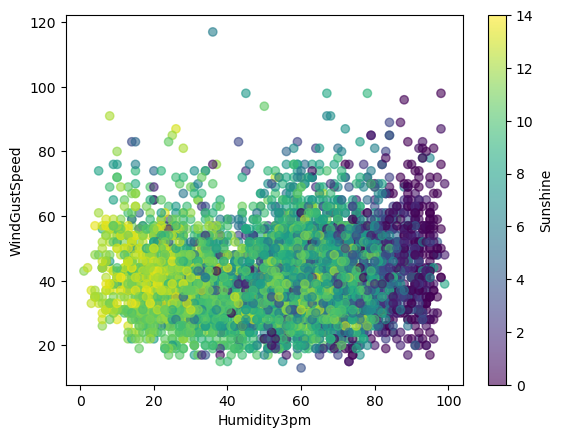
\includegraphics[width=1\textwidth]{Humidity3pm-WindGustSpeed-Sunshine.png}
Examinando o gráfico de dispersão, podemos analisar a relação entre essas variáveis. Parece que não há uma relação linear clara entre 'Humidity3pm' e 'WindGustSpeed', uma vez que os pontos de dados estão espalhados por todo o gráfico. Além disso, a variação de cor devido ao 'Sunshine' indica que diferentes quantidades de sol são registradas para diferentes combinações de umidade e velocidade de rajada de vento.
\caption{Gráfico de dispersão}
\end{figure}

\begin{figure}
\includesvg[width=1\textwidth]{Source.gv.min.svg}
\caption{Gráfico da árvore de decisão}
\end{figure}

\section{Codificar as variáveis categóricas}

Podemos ver que há algumas colunas que são do tipo object, que significa que são variáveis categóricas, como 'Location', 'WindGustDir', 'RainToday' e 'RainTomorrow'. Uma árvore de decisão pode lidar com variáveis categóricas diretamente, mas para facilitar a implementação em Python, vamos usar o LabelEncoder para codificar essas variáveis para valores numéricos. Também podemos ver que há alguns valores ausentes (NaN) nas colunas 'Evaporation', 'Sunshine' e 'Cloud'.

\section{Dividir os dados em treinamento e teste}
Em seguida, dividimos os dados em conjuntos de treinamento e teste. Os dados de treinamento serão usados para treinar o modelo de árvore de decisão, enquanto os dados de teste serão usados para avaliar o desempenho do modelo.

\section{Criar e treinar o modelo de árvore de decisão}
Agora é hora de criar e treinar o modelo de árvore de decisão usando os dados de treinamento. A árvore de decisão é um tipo de algoritmo de aprendizado de máquina supervisionado que pode lidar com variáveis numéricas e categóricas.

\section{Avaliar o desempenho do modelo}
Por fim, avaliamos o desempenho do modelo calculando sua pontuação de precisão nos dados de treinamento. A pontuação de precisão é uma medida que indica a proporção de exemplos classificados corretamente pelo modelo. No caso deste modelo de árvore de decisão, ele alcançou uma precisão de 81\% nos dados de treinamento.

É importante ressaltar que a avaliação do desempenho do modelo deve ser feita em um conjunto de teste separado para obter uma estimativa mais precisa de sua capacidade de generalização.

\bibliographystyle{acm}
\bibliography{sample}

\end{document}